\subsection{Tilbagekobling}
\label{effekt_tilbagekobling}
Tilbagekoblingen har flere opgaver i effektforstærkeren. Den sikrer at den ønskede spændingsforstærkning opnåes i effektforstærkeren. Hvordan dette bestemmes følger senere i dette afsnit. Den bekæmper ulineariteter, afhængig af mængden af tilbagekobling \cite{tilbage-mm1}%\kilde{Palle Andersen, mm1 tilbagekoblingsteori}
. Desuden sørger den for at det faste spændingsfald over $V_\mathrm{BE}$-multiplieren kommer til at ligge korrekt. Dette sker da $V_\mathrm{BE}$-multiplieren laver et DC-offset, som kan komme til at betyde at de to darlingtontransistorer i udgangstrinnet ikke vil være lige åbne. Dermed vil der være en forskel i strømmene igennem dem, hvilket kun kan komme gennem belastningen, hvormed der skabes et DC-offset på udgangen. Som det vises senere i dette afsnit, tilbagekobler tilbagekoblingen DC fuldt, hvormed differensforstærkeren vil sørge for at inputsignalet og outputtet til belastningen kommer til at ligge på samme DC-niveau, hvilket er det der menes med at spændingsfaldet over $V_\mathrm{BE}$-multiplieren ligger korrekt. 

For at regne på tilbagekoblingen til effektforstærkeren er det nødvendigt at kende open-loop forstærkningen, $A$, som er givet ved udtrykket vist i formel (\ref{equ:a-openloop}).

\begin{equation}
\label{equ:a-openloop}
A = A_\mathrm{diff.amp} \cdot \frac{R_\mathrm{i,vol}}{R_\mathrm{o,diff} + R_\mathrm{i,vol}} \cdot \frac{}{} A_\mathrm{vol.amp} \cdot A_\mathrm{cur.amp}
\end{equation}

Spændingsforstærkningen i differensforstærkeren, $A_\mathrm{diff.amp}$, er i afsnit \ref{effekt_differensforstaerker} fundet til 367,6 gange, mens spændingsforstærkningen i spændingsforstærkeren, $A_\mathrm{vol.amp}$, i afsnit \ref{effekt_spaendingsforstaerker} er fundet til 1964,44 gange. Modstanden $R_\mathrm{o,diff}$ er udgangsmodstanden af differensforstærkeren, som i afsnit \ref{effekt_differensforstaerker} er beregnet til 9,56 k\ohm. Modstanden $R_\mathrm{i,vol}$ er indgangsmodstanden af spændingsforstærkeren som er givet ved $R_\mathrm{i,vol} = R_\pi = \frac{h_{fe}}{g_m} = 1,43~\mathrm{k}\ohm$. Denne spændingsdeling er med i formel (\ref{equ:a-openloop}), da der regnes med spændingsforstærkninger. Spændingsforstærkningen i strømforstærkeren, som er en common-collector, $A_\mathrm{cur.amp}$, er givet ved udtrykket i formel (\ref{equ:a-cc})\fixme{kilde: formel 4.96 i sedra smith}, hvor $R_L$ er belastningsmodstanden på 8 \ohm~ i serie med den termiske sikringsmodstand på 0,536 \ohm~ og $r_e$ er en T-model-parameter. Mellem spændingsforstærkeren og strømforstærkeren er der ingen spændingsdeling, da forstærkningen i spændingsforstærkeren, i afsnit \ref{effekt_spaendingsforstaerker}, er beregnet med belastningen fra strømforstærkeren.

\begin{equation}
\label{equ:a-cc}
A_\mathrm{cur.amp} = \frac{R_L}{R_L+r_e}
\end{equation}

T-model-parameteren $r_e$ er givet ved udtrykket i formel (\ref{equ:beta-re})\kilde{afsnit 4.5.7 i sedra smith}.

\begin{equation}
\label{equ:beta-re}
r_e = \frac{\alpha}{g_m} = \frac{\alpha}{\frac{I_C}{V_T}}
\end{equation}

Transistorparameteren $\alpha$ er givet ved udtrykket i formel (\ref{equ:alpha-def}).

\begin{equation}
\label{equ:alpha-def}
\alpha = \frac{\beta}{\beta + 1}
\end{equation}

Det ses af udtrykket i formel (\ref{equ:alpha-def}) at $\alpha \approx 1$, da $\beta>>1$ for BDX33B og BDX34B. Dermed kan $r_e$, for en $I_C$ på de maksimale 2,24 A, bestemmes som vist i formel (\ref{equ:beta-re1}).

\begin{equation}
\label{equ:beta-re1}
r_e \approx \frac{1}{\frac{\mathrm{2,24~A}}{\mathrm{26~mA}}} \approx \mathrm{11,6~m\ohm}
\end{equation}

Resultatet i udregningen i formel (\ref{equ:beta-re1}) leder til en bestemmelse af $A_\mathrm{cur.amp}$ som vist i beregningen i formel (\ref{equ:a-cc-val}).

\begin{equation}
\label{equ:a-cc-val}
A_\mathrm{cur.amp} = \frac{\mathrm{8,536~\ohm}}{\mathrm{8,536~\ohm~} + \mathrm{11,6~m\ohm}} = 0,99
\end{equation}

Open-loop forstærkningen, $A$, kan nu bestemmes som vist i udregningen i formel (\ref{equ:a-openloop-val}).

\begin{equation}
\label{equ:a-openloop-val}
A = A_\mathrm{diff.amp} \cdot \frac{R_\mathrm{i,vol}}{R_\mathrm{o,diff} + R_\mathrm{i,vol}} \cdot \frac{}{} A_\mathrm{vol.amp} \cdot A_\mathrm{cur.amp} = 93022
\end{equation}

Closed-loop forstærkningen, $A_f$, som er givet ved udtrykket vist i formel (\ref{equ:af_def})\kilde{formel 9.4 i sedra smith}, ønskes til 8,95. Dette skyldes at der, som beregnet i afsnit \ref{valg_kortslutningssikring}, skal være 17,9 V over belastningen når der kommer 2 V som input til effektforstærkeren.

\begin{equation}
\label{equ:af_def}
A_f = \frac{A}{1 + A \cdot \beta}
\end{equation}

Da $A$ er bestemt i formel (\ref{equ:a-openloop-val}), kan $\beta$ ud fra udtrykket i formel (\ref{equ:af_def}) bestemmes til 0,11. Med $\beta$ fastlagt, kan mængden af tilbagekobling bestemmes som vist i udregningen i formel (\ref{equ:amountfeedback}).

\begin{equation}
\label{equ:amountfeedback}
1 + A \cdot \beta = 10233
\end{equation}

Med open-loop forstærkningen, $A$, og tilbagekoblingsfaktoren, $\beta$, bestemt, kan følsomheden overfor ændringer i $A$, $S_A^{~A_f}$, desuden bestemmes som vist i udregningen i formel (\ref{equ:a-sens-val}).

\begin{equation}
\label{equ:a-sens-val}
S_A^{~A_f} = \frac{1}{1 + A \cdot \beta} = 0,000098
\end{equation}

Dette betyder at en tænkt ændring i $A$ på f.eks. 20 \% vil give en ændring på closed-loop forstærkning som beregnet i formel (\ref{equ:a-sens-val-diff}).

\begin{equation}
\label{equ:a-sens-val-diff}
S_A^{~A_f} \cdot 20~\% = 0,00002~\%
\end{equation}

Tilbagekoblingskredsløbet opbygges som en spændingsdeler, som vist på figur \ref{fig:beta-clean}, hvormed closed-loop forstærkningen, $A_f$, bliver som vist i formel (\ref{equ:af-deler})\kilde{eksempel 9.1 i sedra smith}.

\begin{figure}[h]
\centering
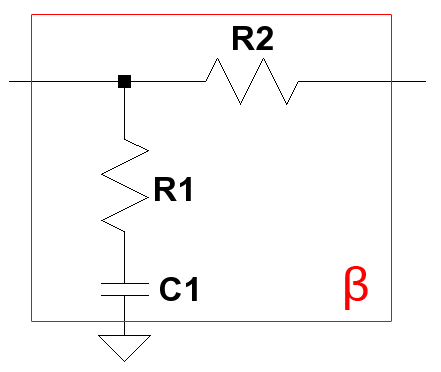
\includegraphics[scale=0.3]{teknisk/effektforstaerker/beta-clean.png}
\caption{Opbygning af tilbagekoblingskredsløb}
\label{fig:beta-clean}
\end{figure} 

\begin{equation}
\label{equ:af-deler}
A_f = \frac{R_1 + R_2}{R_1} = 1 + \frac{R_2}{R_1}
\end{equation}

Dette er gældende så længe $A \cdot \beta >> 1$, hvilket er tilfældet. For at opnå en $A_f$ på 8,95 skal forholdet mellem $R_2$ og $R_1$ altså være 7,95. Kondensatoren, $C_1$, er indsat for at tilbagekoble hele DC-signalet. Dette sker da kondensatoren er en afbrydelse for DC, hvormed udtrykket i formel (\ref{equ:afdc-deler}) beskriver closed-loop forstærkningen for DC.

\begin{equation}
\label{equ:afdc-deler}
A_{f_\mathrm{dc}} = 1 + \frac{R_2}{\infty} \approx 1
\end{equation}

Kondensatoren giver altså den effekt at effektforstærkeren ikke forstærker DC. Størrelsen af kondensatoren beregnes så alle revelante frekvenser ser spændingsdelingen og dens værdi regnes derfor ved én dekade før 20 Hz, altså 2 Hz. Modstanden, $R$, der skal bruges til udregningen af kondensatoren er vist i formel (\ref{equ:r-kondensator}), hvor $R_{i_{Q_2}}$ er den modstand differensforstærkeren belaster spændingsdeleren med, som bestemt i afsnit \ref{effekt_differensforstaerker} til 9,56 k\ohm~, og $R_L$ er belastningsmodstanden på 8 \ohm.

\begin{equation}
\label{equ:r-kondensator}
R = R_1 + R_{i_{Q_2}}||(R_2 + R_L)
\end{equation}

Her ses det at $R_2$ skal være lille hvis betydningen af $R_{i_{Q_2}}$ skal formindskes. Med tommelfingerreglen om omkring en faktor 10, vælges $R_2$ til 795 \ohm, hvormed $R_1$ skal være 100 \ohm. Modstanden $R$ bliver dermed 834 \ohm~ og kondensatorens størrelse bestemmes som vist i udregningen i formel (\ref{equ:kondensator-val}).

\begin{equation}
\label{equ:kondensator-val}
C = \frac{1}{2 \cdot \pi \cdot f \cdot R} = \frac{1}{2 \cdot \pi \cdot \mathrm{2~Hz} \cdot \mathrm{840~\ohm}} = \mathrm{95~\mu F}
\end{equation}

Med denne værdi på plads er alle værdierne til tilbagekoblingen beregnet.